\documentclass{llncs}
\usepackage{graphicx}
\usepackage{subfig}
\usepackage{url}
\usepackage{listings}
\usepackage{authblk}
\usepackage[pdftex]{hyperref}
\usepackage{ifthen}
\usepackage{amssymb}

\newcommand{\TODO}[1]{\textbf{TODO:} \emph{#1} }
\newcommand{\NOTE}[1]{\textbf{NOTE:} \emph{#1} }
% Uncomment the following lines to remove TODO and NOTE labels
\renewcommand{\TODO}[1]{}
\renewcommand{\NOTE}[1]{}

\def\genom{G\textsuperscript{en}oM~}

% proof-reading
\usepackage{xcolor}
\usepackage[normalem]{ulem}
\newcommand{\ra}{$\rightarrow$}
\newcommand{\ugh}[1]{\textcolor{red}{\uwave{#1}}} % please rephrase
\newcommand{\ins}[1]{\textcolor{blue}{\uline{#1}}} % please insert
\newcommand{\del}[1]{\textcolor{red}{\sout{#1}}} % please delete
\newcommand{\chg}[2]{\textcolor{red}{\sout{#1}}{\ra}\textcolor{blue}{\uline{#2}}} % please change
\newcommand{\chk}[1]{\textcolor{ForestGreen}{#1}} % changed, please check

% comments \nb{label}{color}{text}
\newboolean{showcomments}
\setboolean{showcomments}{true} % put to false for the final version
\ifthenelse{\boolean{showcomments}}
	{\newcommand{\nb}[3]{
		{\colorbox{#2}{\bfseries\sffamily\scriptsize\textcolor{white}{#1}}}
		{\textcolor{#2}{\sf\small$\blacktriangleright$\textit{#3}$\blacktriangleleft$}}}
	 \newcommand{\version}{\emph{\scriptsize$-$Id$-$}}}
	{\newcommand{\nb}[3]{}
	 \newcommand{\version}{}}
\newcommand{\pierrick}[1]{\nb{Pierrick}{green}{#1}}
\newcommand{\serge}[1]{\nb{Serge}{blue}{#1}}


\lstset{language=Python, basicstyle=\scriptsize, tabsize=4}

\title{\LARGE \bf Versatile Robotics Simulation Using MORSE}
%\title{\LARGE \bf Evaluation of Robotics Software Using the MORSE Simulator}

%%%%%%%%%%%%%%%%%%%%%%%%%%%%%%%%%%%%%%%%%%%%%
% Standard author list
%%%%%%%%%%%%%%%%%%%%%%%%%%%%%%%%%%%%%%%%%%%%%
%\author[1]{Gilberto Echeverria \thanks{gechever@laas.fr}}
%\author[1]{S{\'e}verin Lemaignan \thanks{slemaign@laas.fr}}
%\author[1]{Arnaud Degroote \thanks{adegroot@laas.fr}}
%\author[2]{Michael Karg\thanks{kargm@in.tum.de}}
%\author[3]{Pierrick Koch\thanks{pierrick.koch@unicaen.fr}}
%\author[4]{Charles Lesire-Cabaniols\thanks{charles.lesire@onera.fr}}
%\affil[1]{LAAS-CNRS, Toulouse, France}
%\affil[2]{TUM, Munich, Germany}
%\affil[3]{GREYC-CNRS, Caen, France}
%\affil[4]{ONERA, Toulouse, France}
%
%\renewcommand\Authands{ and }

%%%%%%%%%%%%%%%%%%%%%%%%%%%%%%%%%%%%%%%%%%%%%
% LLNCS author list
%%%%%%%%%%%%%%%%%%%%%%%%%%%%%%%%%%%%%%%%%%%%%
\author{Gilberto Echeverria\inst{1}\thanks{\email{gechever@laas.fr}}
    \and S{\'e}verin Lemaignan\inst{1}\thanks{\email{slemaign@laas.fr}}
    \and Arnaud Degroote\inst{1}\thanks{\email{adegroot@laas.fr}}
    \and Simon Lacroix\inst{1}\thanks{\email{slacroix@laas.fr}}
    \and Michael Karg\inst{2}\thanks{\email{kargm@in.tum.de}}
    \and Pierrick Koch\inst{3}\thanks{\email{pierrick.koch@unicaen.fr}}
    \and Charles Lesire\inst{4}\thanks{\email{charles.lesire@onera.fr}}
}

\institute{
    CNRS, LAAS, 7 avenue du colonel Roche, F-31077 Toulouse, France
    Universit{\'e} de Toulouse, UPS, INSA, INP, ISAE, LAAS,
    F-31077 Toulouse, France
    \and
    Institute for Advanced Study, Technische Universit\"{a}t M\"{u}nchen,
    Lichtenbergstrasse 2a, D-85748 Garching, Germany
    \and
    UMR 6072 GREYC Universit{\'e} de Caen-Basse Normandie/CNRS/ENSICAEN, France
    \and
    ONERA -- the French Aerospace Lab, F-31055, Toulouse, France
}


\begin{document}
\maketitle

\begin{abstract}
  MORSE is a robotics simulation software developed with the collaboration of
  researchers in several universities. It is a tool to test robotics software
  and algorithms in fairly complex environments. The simulations allow a medium
  to high level of abstraction, to enable researchers to focus on the solution
  of complex tasks.  This is accomplished by connecting directly with the
  robotics software using various existing middlewares, such as ROS, YARP and
  others.
  MORSE makes use of the Blender 3D software to produce realistic looking
  environments with physics simulation.  After three years of development,
  MORSE is a mature tool with a large collection of components.
  It has been developed with the interest of simplifying its integration with
  any robotics architecture used, and thus provides many innovative features:
  ``software-in-the-loop'' connectivity, multiple middleware support,
  configurable components, varying levels of simulation realism, distributed
  multi-node simulation for complex scenes and a human avatar that can interact
  with the robots in the virtual environments.
  We present in this paper the current state of the simulator as well as the
  use cases where it has been used to validate several robotics experiments.
\end{abstract}

%%%%%%%%%%%%%%%%%%%%%%%%%%%%%%%%%%%%%%%%%%%%%%%%%%%%%%%%%%%%%%%%%%%%%%
\section{Introduction}
\label{section:introduction}

Computer simulations are today an essential component in robotics research.
Almost every sort of experiment can be validated in simulation before executing
it on real robots.  For this validation to be useful, the simulation must
provide enough fidelity with respect to the real world, within the requirements
of the experimentation.
Creating a fully realistic simulation would be near impossible, since there are
too many aspects that it would need to handle. This is why there are many
simulators with various capacities, each one created to comply with specific
requirements.

The MORSE simulator we present here is meant as a tool that can be used to test
and evaluate very complex robots performing advanced missions in real life
environments. It does not focus on lower level control of the robot, or the
specific mechanics of its components. In turn, it can provide all the
functionality necessary to evaluate the algorithms that control a robot during
the execution of a mission. This is ideal for testing mission plans, high level
control and multi robot coordination.

The outline of this paper is as follows. Section~\ref{section:othersims}
reviews other robotics simulators with a similar design and use as MORSE.
Section~\ref{section:overview} explains the main design principles of MORSE.
Section~\ref{section:features} is the main part of the article, presenting the
unique features of MORSE, exemplified with the projects for which they were
developed. Finally Section~\ref{section:discussion} gives the conclusion and
future plans for the simulator.

%%%%%%%%%%%%%%%%%%%%%%%%%%%%%%%%%%%%%%%%%%%%%%%%%%%%%%%%%%%%%%%%%%%%%%
\section{Competing Simulators}
\label{section:othersims}

A number of other robotics simulators are available, both commercial and
free. We evaluate here the ones whose functionality is most similar to MORSE:

The Player/Stage/Gazebo\cite{psg-1232} is a well known robotics suite.
It is a full set of tools that include the Player communication layer
and two integrated simulators: Stage \cite{Gerkey03theplayer/stage} is basically a
2D simulator optimised for navigation on flat and closed environments.
One of its advantages is the capability to handle very large numbers of
simplified robots \cite{springerlink:10.1007/s11721-008-0014-4}. However, it is
not ideal for more complex scenarios, specially in 3D space. The more recent
Gazebo \cite{Koenig04designand} was developed to cover these shortcomings.
It has received an important boost in its development with its integration
into the ROS platform, and has thus become the most commonly used robotics
simulator. It integrates very well with ROS and Player, but connectivity with
other middlewares requires additional programming.

The USARSim \cite{usarsim-4209284} shares many design concepts with MORSE. It
was initially developed as a simulator for search and rescue operations, uses
the Unreal Engine gaming platform and is built with the concept of modular
components. It is widely used as an evaluation tool for the well known RoboCup
competitions. However, it uses a custom interface to communicate with external
software and does not support some of the most common robotics middlewares.

Another popular robotics simulator is Webots \cite{Webots04}, which is a
commercial product. It provides a full programming environment to create
customised robots and environments, but its interface is complex to use when
creating new components and robots.
It also has an integrated code editor, but the control programs created in it
must then be converted and transferred to the final robot platform.



%%%%%%%%%%%%%%%%%%%%%%%%%%%%%%%%%%%%%%%%%%%%%%%%%%%%%%%%%%%%%%%%%%%%%%
\section{MORSE Architecture Overview}
\label{section:overview}

% Morse \cite{5980252}

MORSE is developed as a library of Python scripts that run on the Blender Game
Engine (BGE).  The BGE offers a powerful environment for a graphical
application and uses the Bullet physics library.
Objects in the BGE can be completely configured, from physics properties (like
mass, friction coefficients and collision bounding boxes) to event and
behaviour scripts using Python.

The simulation is organised as a main core of control functionality that initialises
and coordinates the events in the BGE, and a collection of components that
can be used to assemble a robot with sensors and actuators.
A variety of communication tools allow each of the MORSE components to connect
with external robotics software through middlewares.
MORSE has support for some of the most commonly used robotics
middlewares nowadays, including ROS \cite{ros-288}, Pocolibs
(\serge{Add a reference}) and YARP \cite{metta|ars06}.
Other middlewares are constantly being added, mainly driven by the needs of new
users. This process is simple, as existing middleware bindings can be used as a
template for the new ones.

MORSE aims to provide a simulation where robotics planning and control can be
evaluated.
\serge{This is not the purpose of every simulation engine ?}
It does not intend to achieve super realistic simulation of individual robotics
components. MORSE sensors and actuators can provide the same data as their real
world counterparts. Some components have multiple variants that can work
at different levels of realism and abstraction. This simplification not only
allows the simulation to be faster, but also permits the robotics researchers
to concentrate on testing higher level algorithms for the completion of the
desired tasks.

Individual components are minimalistic in their functionality and  completely
middleware agnostic. They store the important data that needs to be shared
outside MORSE in a Python dictionary called \texttt{local\_data}. When a
simulation scene is created, the components are linked to middlewares as
specified in a configuration script, and the necessary functionality is added
to the components to be able to transmit/receive data through the middleware.
During a simulation, each component performs its expected task and exchanges
the \texttt{local\_data} with the external software.

\serge{local\_data looks like an implementation trick for me. Is this
  really important to describe this mechanism in the paper ? What are
  the benefits regarding the simulation ?}

The data employed by the components can also be altered through the use of
components called \emph{modifiers}. These provide access to the
\texttt{local\_data} to add noise or change the data as required to match the
data from real sensors/actuators. For instance, transforming the coordinate
frame used by Blender into the Universal Transverse Mercator (UTM) coordinate
system.
The whole data flow in MORSE can be seen in the diagram of
Fig.~\ref{fig:dataflow}.

\serge{Figure 1: Middlewares should be renamed as Middlewares
  connectors, Modifiers should be denote as optional.}

\begin{figure}[ht!]
\centering
    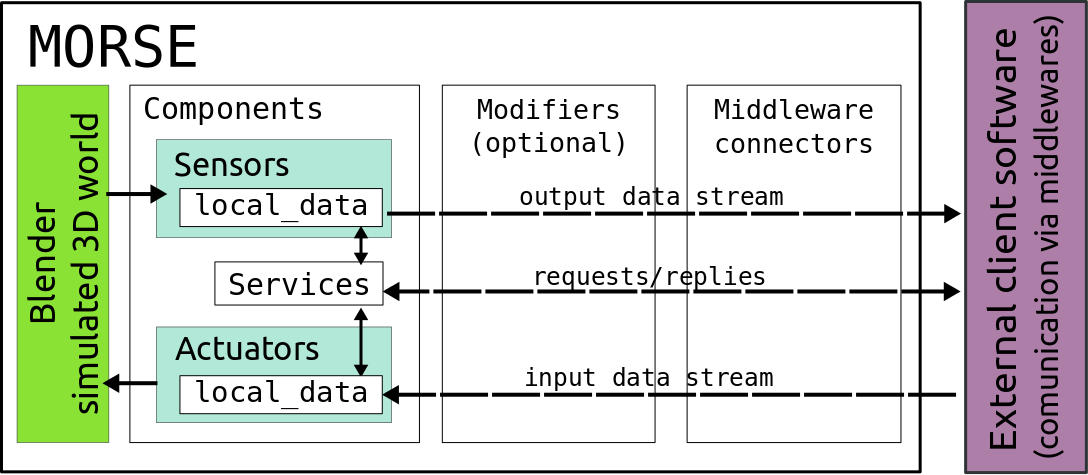
\includegraphics[width=0.8\textwidth]{pics/simulation_main_loop-may2012.png}
\caption{Overview of the data flow in MORSE, between the simulated world
    in Blender and the external robotics software}
\label{fig:dataflow}
\end{figure}

MORSE can be easily extended by adding new components that inherit from the
existing base classes. All components are programmed in Python, since this is
the language that Blender uses for its scripts. However, when coding components
that require a faster processing time, they can be implemented in C/C++, and
then use SWIG to create interfaces that can be included in Python.

An important aspect is that MORSE must be consistent with the execution
logic in the BGE. Python scripts in BGE are executed at a constant
frequency, which is 60 Hz by default in Blender. MORSE components have to
respect this base frequency or run at lower speeds, but not higher. However,
the global frequency in Blender can be increased from the MORSE configuration
scripts.


%%%%%%%%%%%%%%%%%%%%%%%%%%%%%%%%%%%%%%%%%%%%%%%%%%%%%%%%%%%%%%%%%%%%%%
\section{Innovative Features}
\label{section:features}


%-----------------------------------------------%
\subsection{Blender Integration}
\label{section:blender}

Being based on the Blender 3D \cite{blender|web} modelling software, any
object, robot or environment can be created and immediately be made available
to use in MORSE.
Many file formats for 3D models can be imported directly into Blender, further
increasing the range of elements that can be used.
The high level of graphical detail is specially useful for realistic looking
simulations, and very important when doing image processing from simulated
video cameras.
To provide a simulation that is closer to the real life experiments, we have
sought to create detailed models of the buildings and terrain where the
experimentations are carried out. Using Blender it is straightforward to
transform the 2D plan of a building into a 3D model. However, outdoor terrains
for experiments in \emph{field robotics} are more difficult to create by hand.
We have developed additional plug-ins for Blender that can read Digital
Elevation Map (DEM) files and create the 3D mesh. Additionally using aerial
photography for textures creates simulated environments that are very similar
to the real ones.  Figure~\ref{fig:models} shows the modelling capabilities of
Blender being used to create the MORSE robots and an environment created from
DEM data.

\begin{figure}[ht!]
\centering
\begin{tabular}{cc}
 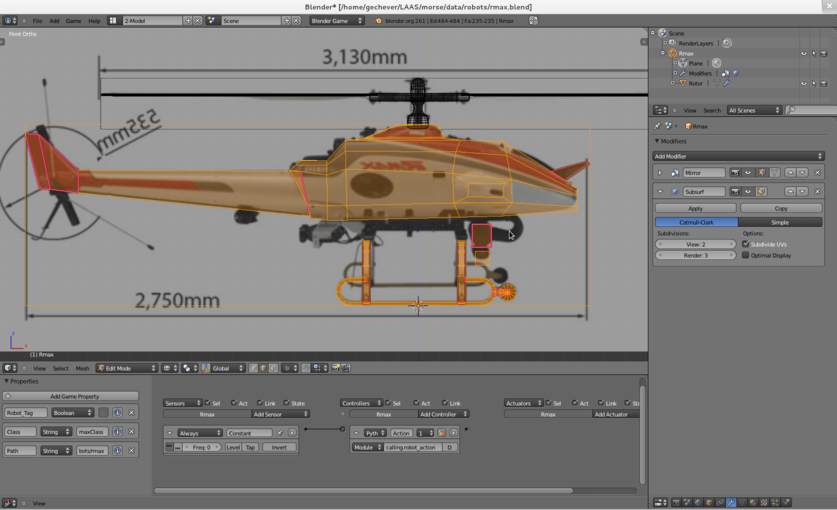
\includegraphics[height=1.55in]{pics/MORSE-rmax_mesh.png} &
 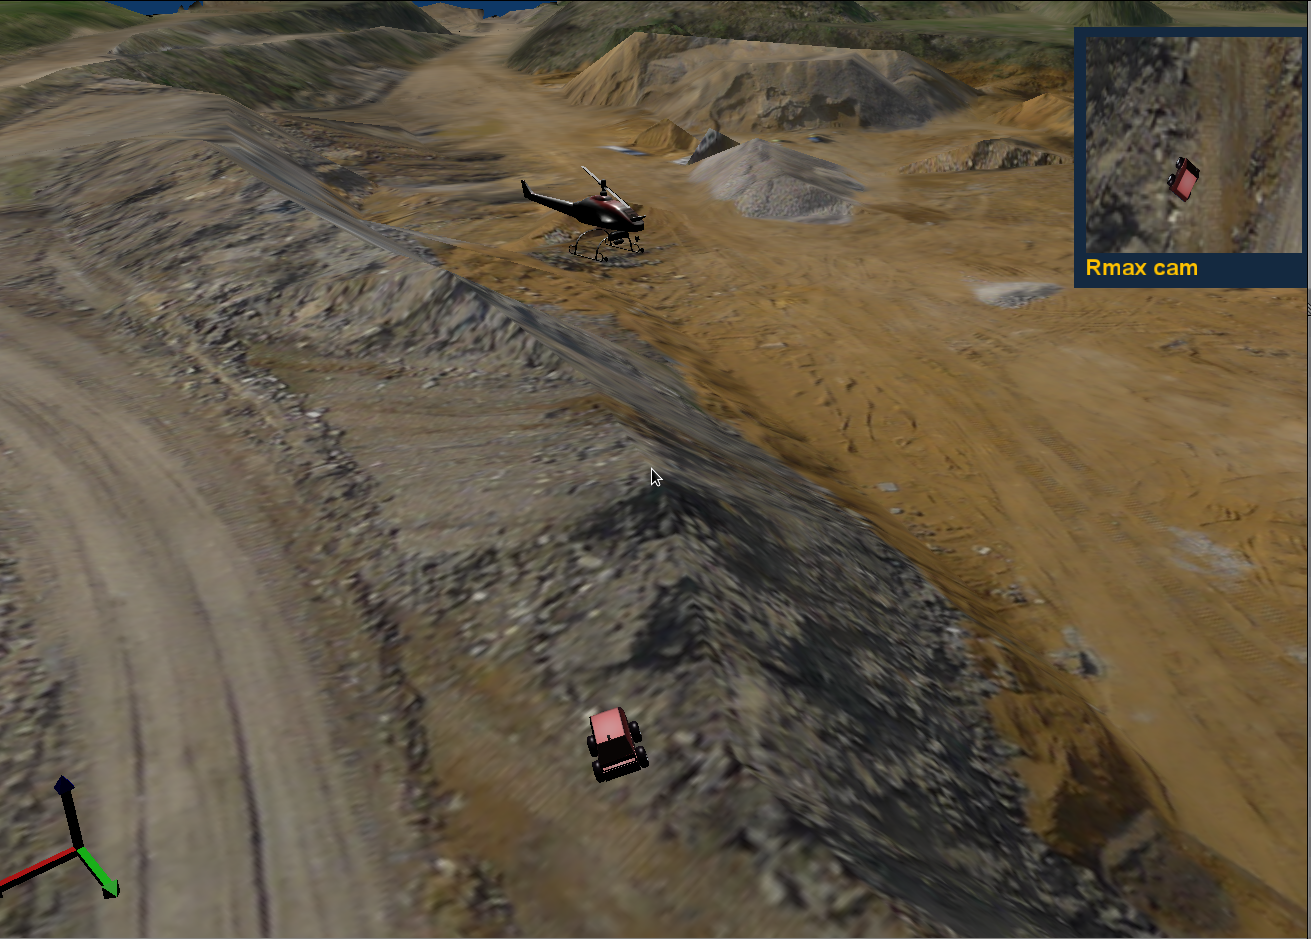
\includegraphics[height=1.55in]{pics/MORSE-quarry_ok-1.png}
\end{tabular}
\caption{Left: Modelling of an R-Max robotic helicopter. Right: Robots on a
    terrain imported from a Digital Elevation Map; the view from a camera mounted
    on a helicopter robot is shown in the top right frame}
\label{fig:models}
\end{figure}


%-----------------------------------------------%
\subsection{Component Library and Scene Construction}
\label{section:components}

To be as versatile as possible, MORSE consists of a collection of components
that can be used to construct robots with various configurations. The
components are classified as:

\begin{itemize}
  \item Robots in MORSE have no behaviours. They are only define by a physical
    shape and properties like mass, friction and collision bounds, which are
    then used by the Bullet physics library to compute the interactions with the
    environment.
    In MORSE, all sensors and actuators must be attached to a robot in order to
    function.
  \item Sensors recover data from the simulated world and store it. This is
    done using the Blender predefined interfaces for the BGE and Python scripts.
    For example, a GPS will read the absolute coordinates of the sensor in the
    Blender world, laser scanners use ray tracing operations to detect
    obstacles and cameras use renders from the perspective of the camera to
    produce images. Parameters that determine how the sensors gather data can
    be adjusted, such as range, resolution, image sizes, etc.
  \item Actuators are charged with carrying out actions within the simulated
    world. There are actuators to provide motion to the robots through several
    methods and algorithms, or to control moving parts such as robotic arms or
    pan-tilt units. In most cases, the motions are implemented using the
    functions in Blender to add a certain linear and angular speed to an
    object.
    Robotic arms consist on a series of articulated segments, and use the
    Blender armature system to determine the degrees of freedom at each joint.
    They can be operated either by direct control of the angles at each joint
    or by control of the end effector with Inverse Kinematics (using the iTaSC
    \cite{iTaSC}, an constraints-based IK solver available for the BGE).
\end{itemize}

The component library also includes other objects that can be used in the
simulation, from large outdoors environments, to furniture and small items.
All of these can be imported from individual Blender files into a simulation
scenario.

Building and configuration of scenarios are done with a set of Python
classes provided by MORSE, known as the \emph{Builder API}. It completely hides
the interface of Blender from the user, so that those unfamiliar with Blender
can directly configure MORSE using Python scripts. Scripts can then be tracked
on a version control system to follow changes and apply patches.
The API offers classes to add robots, sensors and actuators, to position,
rename and configure any of the parameters used by these components, to
include additional objects (furniture, obstacles, etc.) and to add middleware
bindings, modifiers and services for each component.
%When executing MORSE, the Builder API will create a new Blender file with all
%the parameters necessary to run the simulation. Afterwards, when the BGE is
%started, it will use the parameters given to the components to produce the data
%in the simulation.

MORSE has been chosen as the simulator platform for a french research
robotic project called
\emph{ANR-PROTEUS}\footnote{\url{http://anr-proteus.fr/}}, thanks to
its versatility and the facility to integrate it with
existing architectures.

The PROTEUS project supports a model-driven engineering approach based on a
domain-specific language and a robotic ontology\cite{Dhouib:2011zr} and aims at
providing a toolchain for robotic development from modeling to software
simulation and deployment on real robots. PROTEUS is based on open-source
softwares like the Eclipse Modeling Project, the ROS middleware and MORSE
simulator. Several robots modeling are currently under construction (Wifibot,
ECA Camelon, and Thales R-Trooper).

%-----------------------------------------------%
\subsection{Adjustable Levels of Realism}
\label{section:realism}

Many components come in several versions, which produce more or less
realistic behaviour, and can be chosen depending on the objective of the
simulation and the treatment that will be given to the data.

Land robots can have realistic wheel behaviour and physics, or be handled as
rigid boxes sliding over the ground. For aerial and submarine robots, the
physics are limited to collision detection, but they are not affected by
gravity, and there is no simulation of air or wind currents.

Some sensors provide the same kind of raw data as their real counterparts,
which can then be processed to extract relevant information,
and later used to take decisions. When the processing of data is not of
interest to the experiment, alternative sensors can be used which provide
higher level data, extracted directly from the BGE scenario, and avoid costly
processing.
The clearest example of this are the cameras: the regular video camera
generates renders of the Blender scene, and outputs images to be processed by
software. This generates too much data, and can slow down the simulation when
rendering for several cameras at once. A new sensor called the \emph{semantic
camera} uses Blender functions to determine the names and location of the
objects within the view frustum of the camera. It outputs this data and avoids
two steps of processing, making the simulation (up to 100\%) faster and
avoiding image processing algorithms.

The same is true for actuators, which offer the choice between controlling the
speeds of wheels independently, controlling the motion of the robot as a whole
with linear and angular velocities, giving direct waypoint coordinates for
destination (even using a very basic obstacle avoidance mechanism), or
``teleporting'' a robot to the desired location.

This flexibility permits scientists to focus on specific problems, instead of
juggling with many algorithms running at once.
\serge{I don't understand the point here.}

For instance, researchers from ONERA use MORSE to evaluate online probabilistic
decision-making on an autonomous UAV. In a first scenario~\cite{teichteil2011},
MDP-based policy optimization allows the UAV to find a suitable zone for an
emergency landing. MORSE video camera sensors are used to feed the raw image data
into the land mapping algorithm.
On a second scenario~\cite{carvalho2012}, a POMDP model is used to optimize the
probability to track and intercept an identified target among others. As the
objective of simulations is to evaluate the optimized strategy, processing
simulated images is not necessary. Hence, instead of using a video camera
sensor, they use the ``semantic camera'' to get the location of the target,
adding some noise with modifiers to simulate both the sensor and the detection
and identification process.

\serge{Semantic Camera and Components overlays should be emphasized as
  two new mechanisms of MORSE. Could we add more information on how
  Semantic Camera works ?}

\serge{Regarding the adjustable level of realism, you should talk
  about the SEGWAY model available now in MORSE, as an example of a
  very accurate physical model compared to the basic ones.}

%-----------------------------------------------%
\subsection {Middleware Configurations}
\label{section:middlewares}

Many research laboratories use different interfaces to communicate with their
robots. In order to be usable with any architecture, MORSE enforces a
clear separation between MORSE components and middlewares. When a simulation is started,
the bindings between sensors/actuators and middlewares are read from the
configuration script, and it is only then that components acquire the functions
necessary to communicate with the outside world.
This separation means that any middleware can be integrated with MORSE, by
simply providing the scripts to marshal MORSE data in the expected format.
Middlewares currently supported include ROS, MOOS, Pocolibs, YARP and
TCP/IP sockets.
Information exchange between the simulator and the robotics software can be
done by a constant data stream, or via request/reply interfaces.

MORSE permits using many different middlewares within a single simulation
scenario. This is exemplified in the \emph{Action project} \cite{6106782}
developed by the LAAS and ONERA labs.
It consists in the cooperation of ground and air robots to patrol a zone,
locate and follow moving targets.
Each lab provides an existing robotics platform with very different
architectures: LAAS employs Segway RMP 400 land robots, using the \genom
\cite{MALLET-2011-599677} architecture, while ONERA works with Yamaha R-Max
helicopters based on Orocos \cite{orocos2003}. The simulation uses Pocolibs to
communicate with \genom, and YARP to talk with OROCOS.

The use of simulation is particularly beneficial for this project, since the trials
are done in a very specific environments, and require transporting the robots a
considerable distance, always being dependant on the prevailing weather.
Software evaluation can be done in MORSE regardless of the weather, and not
having to plan long trips to the actual experimental site.
Simulation also simplifies the execution of test runs, since they can be
restarted from the initial point within seconds.  Future stages of the project
require the coordination of larger teams of heterogeneous robots. The physical
robots required for these stages are not currently available, but simulation
permits for testing of these scenarios in advance.


%-----------------------------------------------%
\subsection{Component Overlays for Specific Architectures}
\label{section:overlays}

\serge{What is architecture here ? Existing software architecture,
  hardware ?}
\serge{Component overlays could be seen as an implementation of the
  adapter Pattern: \url{https://en.wikipedia.org/wiki/Adapter_pattern}}

Besides the existing variety of components and middlewares available, it is
further possible to adapt these elements to better fit an existing
architecture and allow true ``software-in-the-loop'' functionality.

MORSE components provide dedicated I/O interface. In
many cases, the interface methods will not be the same as those used in an
actual device, although the component has the same functionality.
For instance, an actuator may have two separate functions to modify its linear
and angular velocities, while the corresponding MORSE component uses only one
function with the two parameters. To avoid creating additional components,
MORSE implements the notion of \emph{component overlays}. These are
special pseudo components that override the default
behaviour to make it match a different architecture.
In the case of middlewares, it is possible to either use the default
serialization methods provided by MORSE, or write additional serialization
functions as extra scripts, specific for single components.
Overlays are implemented as Python scripts that provide an interface between
the real component being simulated and the equivalent sensor available in
MORSE.

These features have been used to connect MORSE with an existing
Unmanned Aerial Vehicle (AUV) control architecture~\cite{barbier2011}
without modifying the code in either the original architecture or MORSE.
%Overlaying the components and middleware serialisations yields these results:
%\begin{itemize}
%  \item the middleware used is based on sockets; while the default MORSE socket
%    middleware serializes the component data one after the other, it has been
%    possible to match the quite complex protocol used in~\cite{barbier2011} by
%    providing custom functions in Python
%  \item the control of the robot is done by providing waypoints to actuators; a
%    specific mechanism that consists in following a path defined by two 3D
%    points, has been obtained by overlaying the default waypoint actuator of
%    MORSE, without having to code any interface component between MORSE and
%    our architecture.
%\end{itemize}


%-----------------------------------------------%
\subsection{Multi-node and Hybrid Simulation}
\label{section:multinode}

\serge{There is no reference to HLA here. I think this is a major
  advance that should be cited appropriately.}
The simulation of multiple robots in the complex environments permitted by
MORSE is very demanding on computational and graphics resources.
A scenario with several robots, video cameras and
other sensors, plus the robotics software all running on the same computer will
slow down the system considerably. MORSE offers the possibility of running
multiple instances of the same simulation scenario in separate computers, but
coordinated by a central server program, called the \emph{multi-node
manager}. While all nodes show all of the robots, each node will only
be charged with controlling a few robots. The movements
of robots and specific objects in one node are sent to the multi-node
manager, which in turn collects the updated positions across all nodes
and redistributes the information, so that all nodes can immediately
reflected the changes. The multi-node server is also charged with
synchronising the time and events across all nodes. It can also be used
to slow down the simulation in all nodes, by making them wait for the
synchronisation message. However, at the current time it is not possible to
accelerate the simulation speed.

This functionality was developed for applications that require a large amount
of robots. Our use case is another outdoors robotics project: \emph{Rosace}
\cite{springerlink:10.1007/978-3-642-12384-9_18,springerlink:10.1007/978-3-642-28786-2_32}.
Its main objective is the coordination of robotic agents in search and rescue
operations in the case of a disaster. In this scenario, terrestrial robots must
be able to locate human victims, provide support for the victims and avoid
dangerous areas. The robots in the team are to be equipped with different
payloads, and take autonomous decisions on which of them should perform
different tasks in the mission, such as searching, providing a communications
relay, and helping victims directly.

For this project, two or three robots can be handled by a single simulation
node, and synchronised with those in other nodes. The communication between the
robots is handled outside the simulation, using specific sensors to simulate
loss of connectivity due to occlusion or distance between the robots.
\serge{The communication is handled outside the simulation by using
  some simulated sensors ? There is a contradiction somewhere ?}

The victims to be saved are internally considered as robots with scripted
behaviour, so that their status and position is also synchronised by the
multi-node manager.

Additionally, the multi-node system permits the deployment of hybrid
simulations. A 3D environment that closely represents the real experimentation
site is used. Real life robots report their updated positions to the multi-node
server, and this last one changes the position of a dummy robot representation
in simulation, so that other simulated robots can see it and interact with it.
In the Action project, a real land robot moves around while the simulated
helicopter can follow it using video cameras.
The robots communicate in the same way they do either in full simulation or in
real life.  The land robot will not be able to ``see'' the simulated helicopter
with its cameras, but in this experiment that is not necessary, since even in
real life the land robot is not capable of seeing the helicopter.

\serge{Maybe this paragraph should emphasized that heterogenous physical simulations
  could be coupled very easily thanks to the HLA support.}

%-----------------------------------------------%
\subsection{The Human Avatar}
\label{section:human}

For human-robot-interaction scenarios, we require a way to combine the
reactive and sometimes unpredictable behaviour of a human interacting with its
environment with a simulated robot. Therefore the human avatar of the MORSE
simulator has been equipped with an intuitive control that enables users to act
upon the simulated environment. Inspired by modern 3D-computer games, the user
takes a third-person perspective behind the human avatar to move around like
shown in Fig.~\ref{fig:human_control} on the left.
While moving around, the camera tries to avoid the objects and walls placed
between the camera and the human avatar to prevent occlusions.  All objects
that can be interacted with can be displayed by pressing a key on the
keyboard (also illustrated in Fig.~\ref{fig:human_control}). When the user
decides to interact with an object, the camera switches to a first-person
perspective and offers an interface showing possible actions the
user can take when pointing to specific objects, as shown in Fig.~
\ref{fig:human_control} on the right. Those actions at the moment include
picking up and releasing objects, opening and closing drawers and cupboards and
switching on and off specific objects like a light or an oven.

\begin{figure}[ht!]
\centering
\begin{tabular}{cc}
 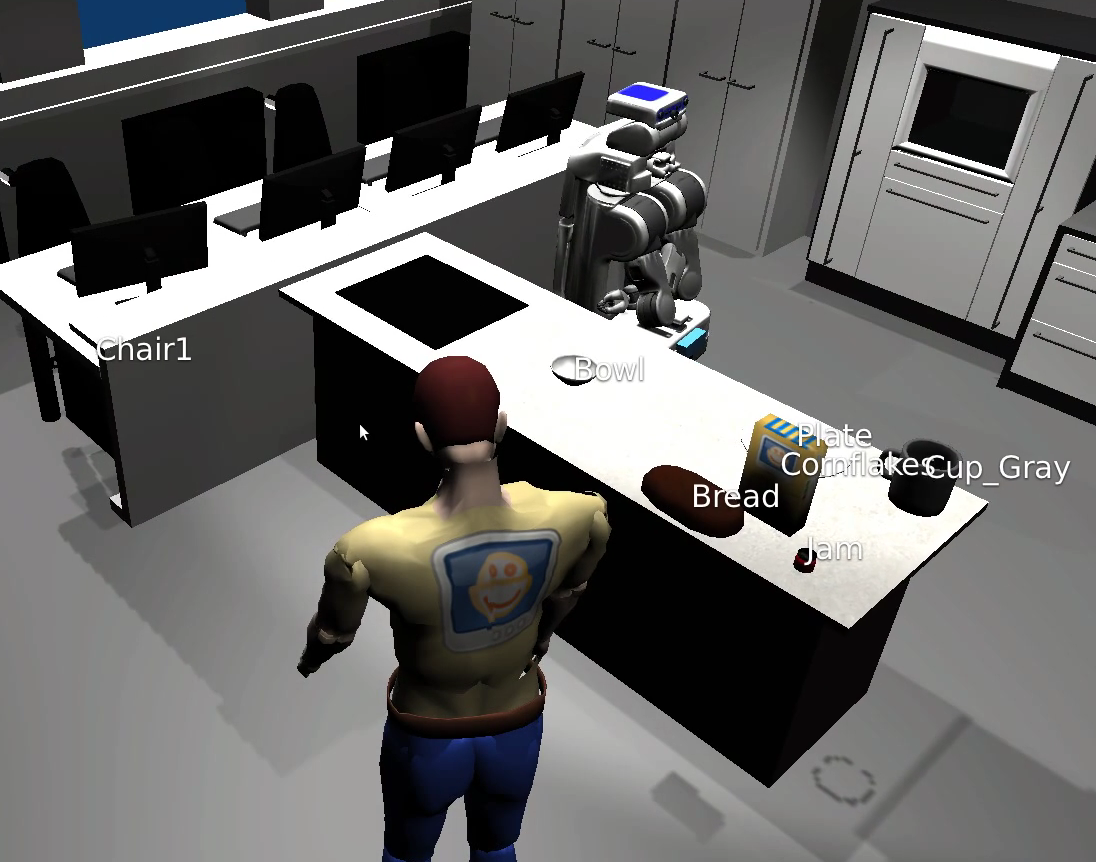
\includegraphics[width=0.475\textwidth]{pics/human_control_1.png} &
 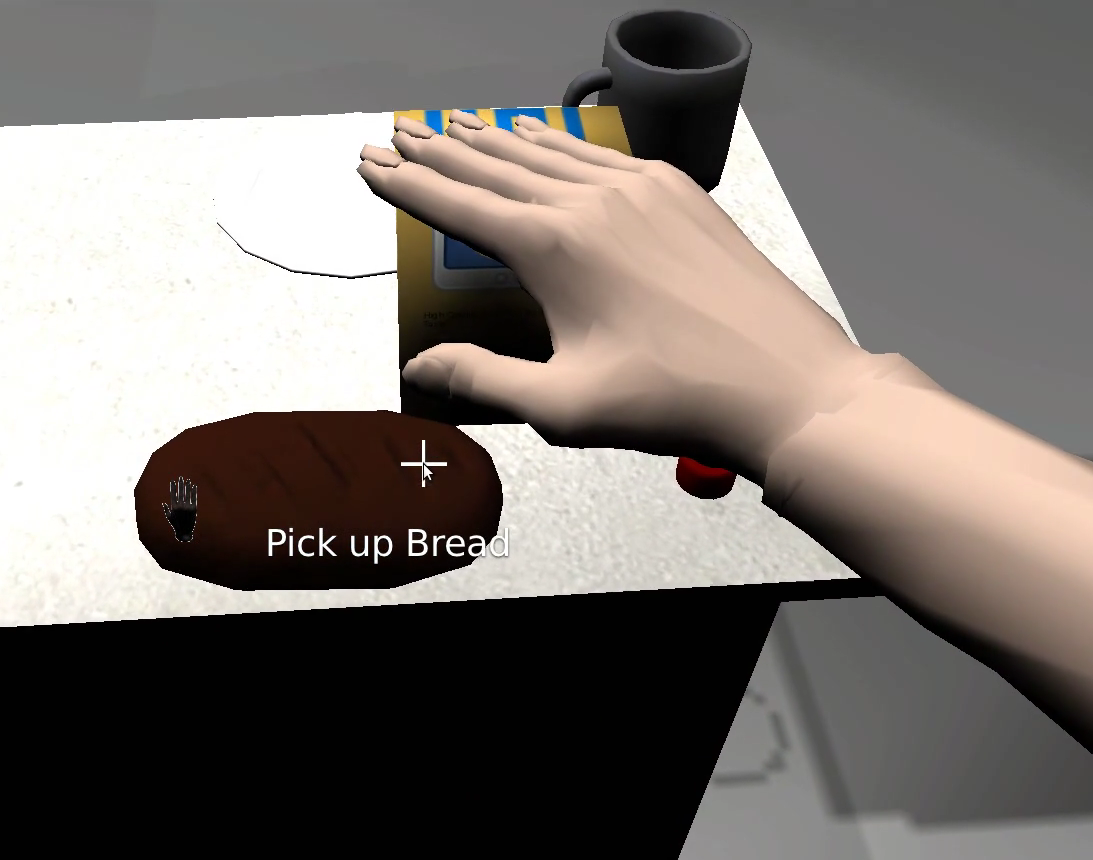
\includegraphics[width=0.475\textwidth]{pics/human_control_2.png}
\end{tabular}
\caption{The left picture shows a third-person view of the human component that
    is used to navigate in the environment. Here objects, that the human can
    interact with, are displayed. The right picture shows the first-person
    perspective of the human avatar that indicates a possible
    ``pick-up-action'' with the bread.}
\label{fig:human_control}
\end{figure}

The motions of the avatar are animated using Blender functionality such as
armatures, Inverse Kinematics, and predefined movement loops.
The avatar can be controlled much like a character in a videogame, using either
the mouse and keyboard or a combination of the Microsoft Kinect and the
Nintendo Wiimote. This computer-game like control enables users to perform
pick and place actions in simulated worlds while at the same time the
simulated robot(s) can be controlled through the supported robotic middlewares.

% TODO: Add picture of kinect/wiimote control

The human avatar is meant to be used in \emph{indoor service robotics} scenarios.
In these, complex robots are expected to collaborate with humans to carry out
ordinary household tasks, such as cleaning, serving food or aiding humans to
navigate an environment.
Robots used in these experiments are equipped with one or two arms, and are
capable of grasping objects. They are also expected to react to the actions of
their human collaborator, using video cameras, motion detectors or telemetry to
determine the location, pose and attitude of the human.
This can be done at two different levels of
abstraction. Using the video cameras to recognise the human and its pose can be
done realistically, with the associated computational cost and uncertainties.
Alternatively, the avatar can directly export the position of all of its
joints, and feed them back to the robot, simulating a full motion capture
system and avoiding the processing costs.


An example use case in this scenario is the testing and validation of human-aware
navigation planners of service robots in human-centred environments at TU Munich.
In this case, a simulated human tracking system provides the human pose to the
robot while the robot navigates in the environment in a way that is safe and
legible for the human. In this project, MORSE has not only been used as a
powerful tool for testing human-aware navigation strategies before carrying out
experiments with real humans. It was also used for their evaluation as
Lichtenth{\"a}ler et al. show in \cite{lichtenthaeler2012increasing} by
video-based user studies. After successful testing and evaluation, the
human-aware navigation was applied using real robots and humans resulting in
a safe and reliable behaviour of the robot.

In another project at TU Munich, a simulated kitchen environment is used
to test and evaluate a plan recognition and monitoring system using the
semantic camera of MORSE as a simulated object recognition system with
a reactive robot control system.
\serge{A missing reference ?}


%%%%%%%%%%%%%%%%%%%%%%%%%%%%%%%%%%%%%%%%%%%%%%%%%%%%%%%%%%%%%%%%%%%%%%
\section{Summary and Future Work}
\label{section:discussion}

We have presented the new features developed on the MORSE simulator,
following the requirements of a variety of projects in robotics research.
The design and architecture of MORSE has proved to be flexible and powerful
enough to allow researchers to use it under various circumstances to test their
robotics algorithms. The development process is simple, and users can customise
many features according to their needs.
All new developments done on top of MORSE are made available to the whole
community, thanks to the open source licence of the simulator.

MORSE allows for quick integration with an existing architecture (multiple
middlewares, modular components and component overlays), heterogeneous robots
(mixing components and middlewares), multiple robot simulation (multi-node
synchronisation) and human-robot interaction (high abstraction level sensors
and human avatar).

Further work is planned to increase the usefulness of MORSE in robotics
experiments:
When doing human-robot interface experiments, it is ideal to have a higher
immersion when using the human avatar.  A planned feature is to provide stereo
images of the simulation to the user wearing special goggles. This can be done
from Blender, with some separation of the images produced for the two eyes.
Further integration with motion reading devices, such as Microsoft Kinect can
also make the experience more natural, by allowing a finer control over the
human avatar.

MORSE is developed as an open--source project with a BSD 3-clause license.
User documentation and additional information is also available at:
(\url{http://morse.openrobots.org})
The source code can be downloaded from the GIT repository:
(\url{http://github.com/laas/morse.git})

\subsubsection*{Acknowledgments}
This work has been partially supported by the DGA funded Action project
(\url{http://action.onera.fr}), the STAE foundation Rosace project
(\url{http://www.fondation-stae.net}) and the ANR-PROTEUS
project (\url{http://anr-proteus.fr/})

% ---- Bibliography ----
% \bibliographystyle{unsrt}
\bibliographystyle{splncs03}
\bibliography{./morseBiblio,charles}
\end{document}
